\section{Ground State Properties}
\vspace{10pt}
Our analysis of the discrete Schrödinger ground state reveals key insights into the connection with Riemann zeros.

\begin{figure}[h]
\centering
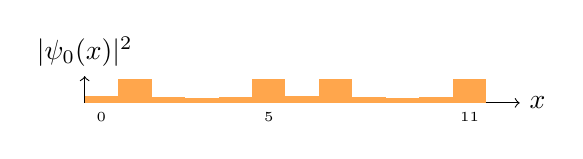
\begin{tikzpicture}[scale=0.85]
    % Draw psi_0^2
    \draw[->] (0,0) -- (6.5,0) node[right] {$x \modm$};
    \draw[->] (0,0) -- (0,0.4) node[above] {$|\psi_0(x)|^2$};
    
    % Draw the ground state probability density
    \foreach \x/\v in {0/0.05, 1/0.18, 2/0.045, 3/0.04, 4/0.045, 5/0.18, 6/0.05, 7/0.18, 8/0.045, 9/0.04, 10/0.045, 11/0.18} {
        \fill[orange!70] (0.5*\x, 0) rectangle (0.5*\x + 0.5, \v*2);
        
        % Label selected x values
        \ifnum\x=0
            \node[below] at (0.5*\x + 0.25, 0) {\tiny \x};
        \fi
        \ifnum\x=5
            \node[below] at (0.5*\x + 0.25, 0) {\tiny \x};
        \fi
        \ifnum\x=11
            \node[below] at (0.5*\x + 0.25, 0) {\tiny \x};
        \fi
    }
\end{tikzpicture}
\caption{Ground state probability density $|\psi_0(x)|^2$ of the discrete Schrödinger equation, showing concentration in prime-rich residue classes.}
\label{fig:psi0}
\end{figure}